\section{Tutorial 1: Creating a First Mesh}

\begin{figure}
\begin{centering}
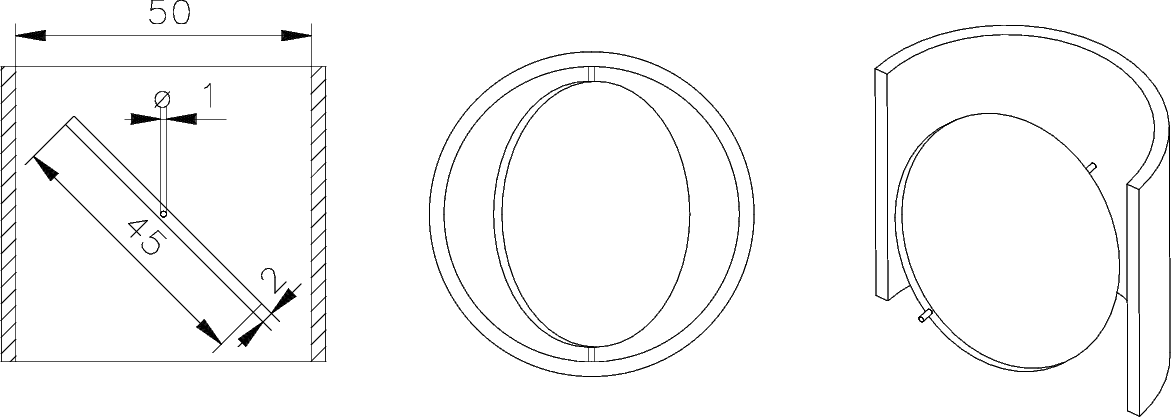
\includegraphics{figures/Throttle}
\par\end{centering}
\caption{Throttle geometry}
\label{fig:throttle1}
\end{figure}

\subsection{Description}

This tutorial will demonstrate how to read a surface mesh and create a volume mesh for a CFD simulation. Figure \ref{fig:throttle1}shows the geometry which will be used for this tutorial; it represents an adjustable throttle. The file containing the surface mesh for this tutorial is called \sqt Throttle.msh\eqt and it can be downloaded from the \eg download page. 

\subsection{Importing the Surface Mesh}
To start, please import the file choosing 

\menu{Import \arr Gmsh \arr v2.0 (ASCII)}

from the menu bar. A file-dialogue will show and you can browse for the file and open it. Figure \ref{fig:T1_scr01} shows a screen-shot of \eg after importing the file. You can use the mouse to rotate, move, and zoom the view. This mouse interaction is the default mouse interaction provided by VTK.

\eg colours the faces of the surface grid in order to determine which side of the surface is inside a flow domain and which is outside. The outside is coloured in a pale green, but figure \ref{fig:T1_scr01} shows pale yellow; this means the surface is wrongly oriented and it needs to be corrected. To do this, please choose 

\menu{Mesh \arr change surface orientation}

from the menu-bar. Afterwards the surface will be oriented correctly.


\begin{figure}
  \begin{centering}
    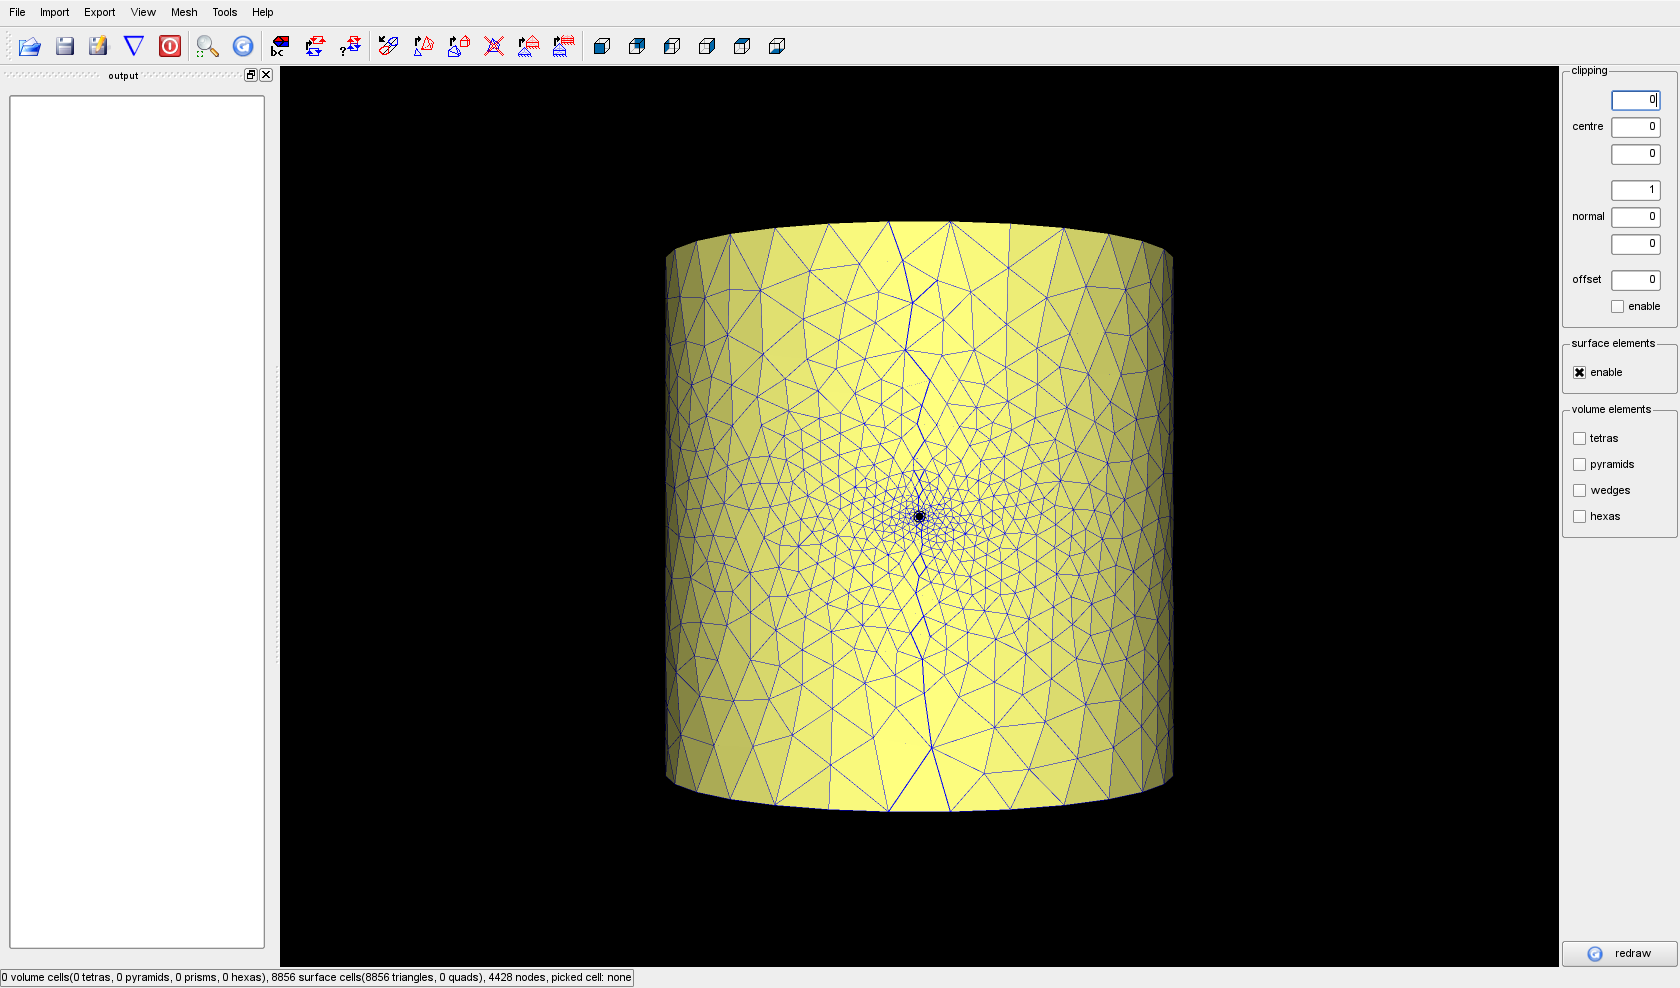
\includegraphics[width=14cm]{figures/tutorials/T1/scr01}
    \par
  \end{centering}
  \caption{After importing the surface mesh}
  \label{fig:T1_scr01}
\end{figure}

\subsection{Defining Boundary Conditions}
Unfortunately all faces belong to the same boundary condition and thus it is not possible to see inside the domain. To change this you can pick a surface on the side of the cylindrical geometry and then change its boundary condition to a different value. To pick a face, please point the mouse over a triangle and press the {}``P'' key on your keyboard. Afterwards you should see something similar to figure \ref{fig:T1_scr02}. To change the boundary code, please select 

\menu{Mesh \arr set boundary code}. 

A small dialogue will pop up and it offers to select a feature angle and a new boundary code. The new boundary code should be set to \sqt 2\eqt and the feature angle can remain at 45 degrees. With this setting you should set the whole side of the cylinder to a new boundary code and the faces should disappear, because they have not been selected for viewing yet. Now, do the same with the top (boundary condition 3) and the bottom (boundary condition 4) of the cylinder. To get rid of the red box, please point the mouse into an empty space and press {}``P'' again. Now would be a good time to save your work. Select 

\menu{File \arr Save Grid As}

to save the file. 

\begin{figure}
  \begin{centering}
    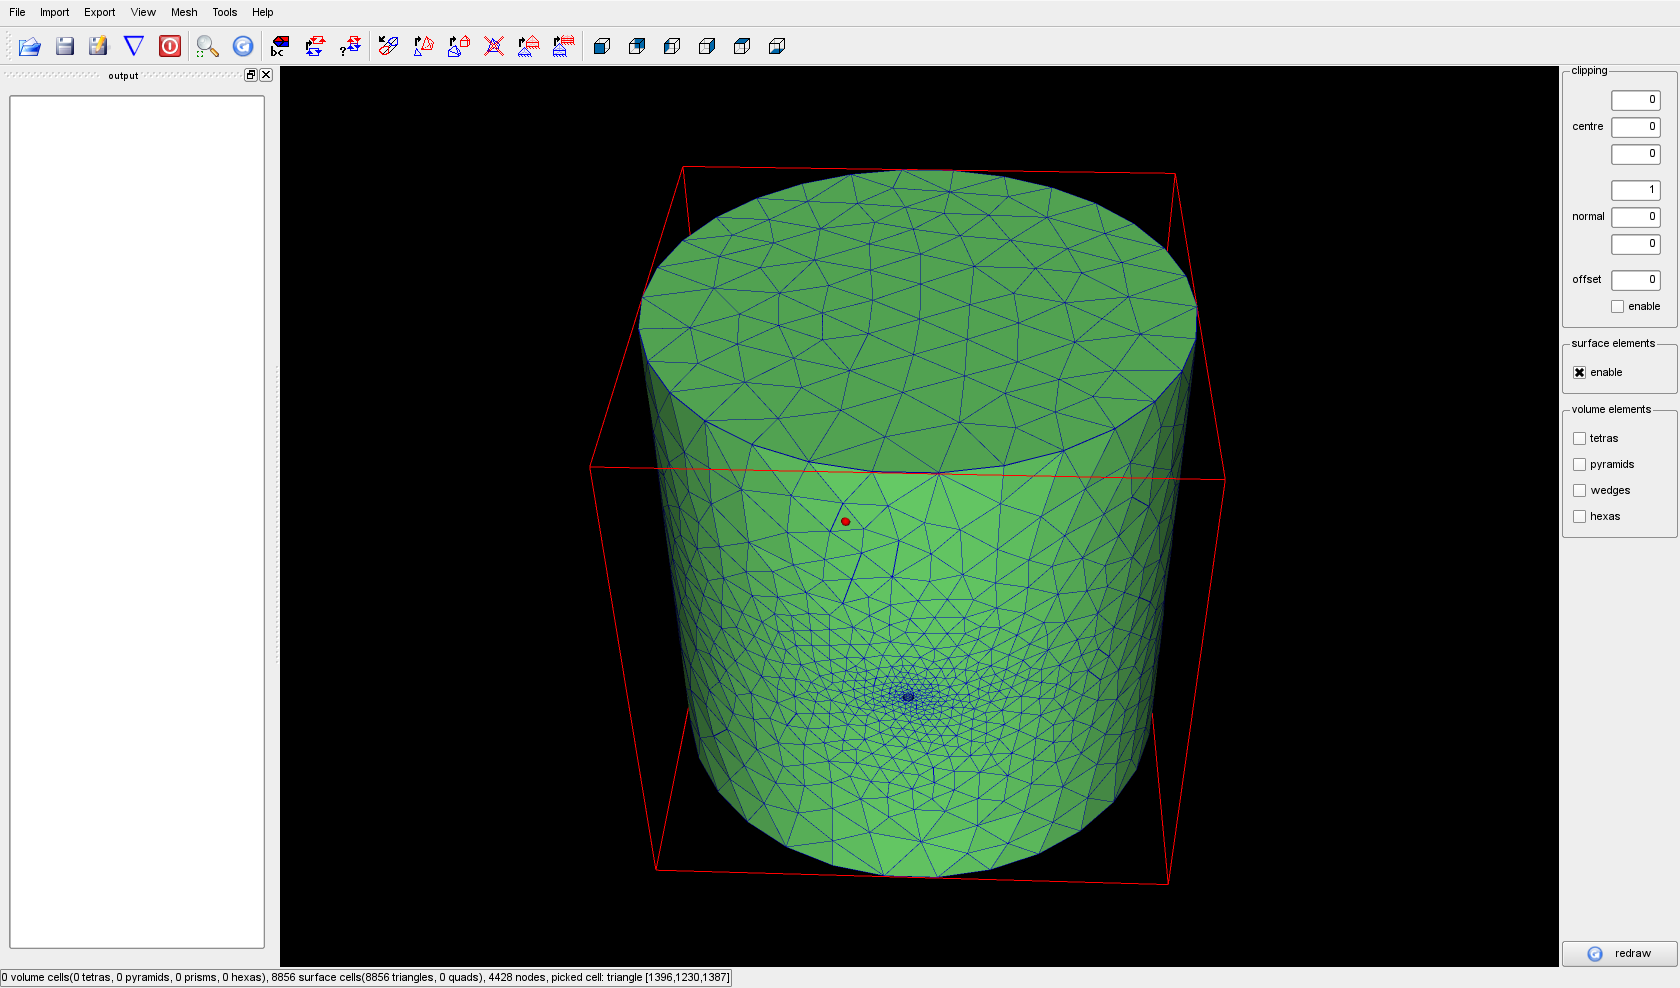
\includegraphics[width=14cm]{figures/tutorials/T1/scr02}
    \par
  \end{centering}
  \caption{After picking a face}
  \label{fig:T1_scr02}
\end{figure}

\begin{figure}
  \begin{centering}
    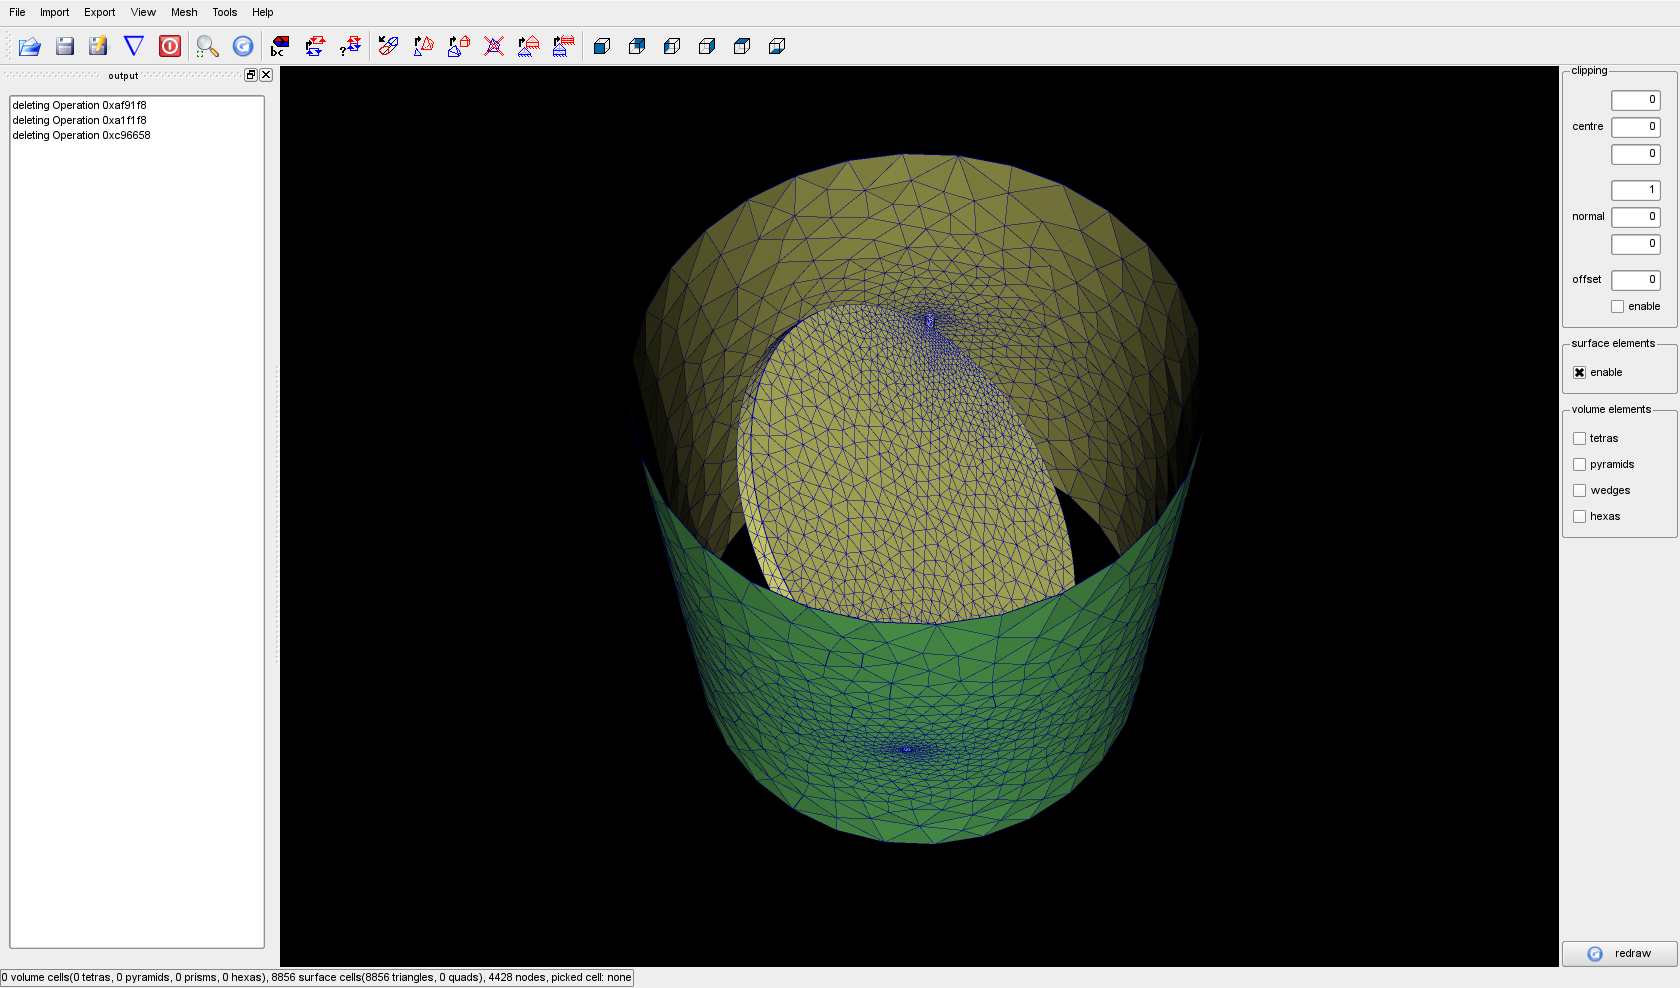
\includegraphics[width=14cm]{figures/tutorials/T1/scr03}
    \par
  \end{centering}
  \caption{Physical walls for prismatic boundary layer}
  \label{fig:T1_scr03}
\end{figure}

\clearpage
\subsection{Create Volume Mesh}
Creating a first volume mesh, including the boundary layer, is fairly easy now. First choose

\menu{View \arr boundary codes}
 
and select the boundary conditions 1 and 2, because these represent the physical walls of the geometry. You should now have something similar to figure \ref{fig:T1_scr03}. To create the grid, simply select

\menu{Mesh \arr create prismatic boundary layer}, 

select the boundary conditions 1 and 2 and click {}``OK''. You can watch the progress in the output window on the left side of the screen. This output window can be detached, moved somewhere else, or hidden completely. \eg indicates that it is busy in the status line at the bottom of the window. After \eg has finished you can select {}``tetras'' and {}``wedges'' from
the available options on the right side of \eg's main window. In order to see inside you should also enable the clipping options. The origin of the clipping plane can be set to (0,0,0) and the normal vector to (0,0,-1). If you now select to view only boundary condition 1 and choose

\menu{View \arr redraw}
 
your screen should look similar to figure \ref{fig:T1_scr04}. To get a nice tetrahedral part of the grid it is advisable to execute

\menu{Mesh \arr create improve volume mesh (NETGEN)}

once or twice. The mesh size distribution is not ideal for the first run of NETGEN. \eg uses an existing volume grid to compute a mesh size distribution and uses this as input for the next call of NETGEN. Normally you get a rather coarse tetrahedral grid together with the prismatic layer. The next call will produce a grid that might be somewhat too fine. Starting from the second call of

\menu{Mesh \arr create improve volume mesh (NETGEN)}
 
the grid should look rather nice (see figure \ref{fig:T1_scr04}).

\begin{figure}
  \begin{centering}
    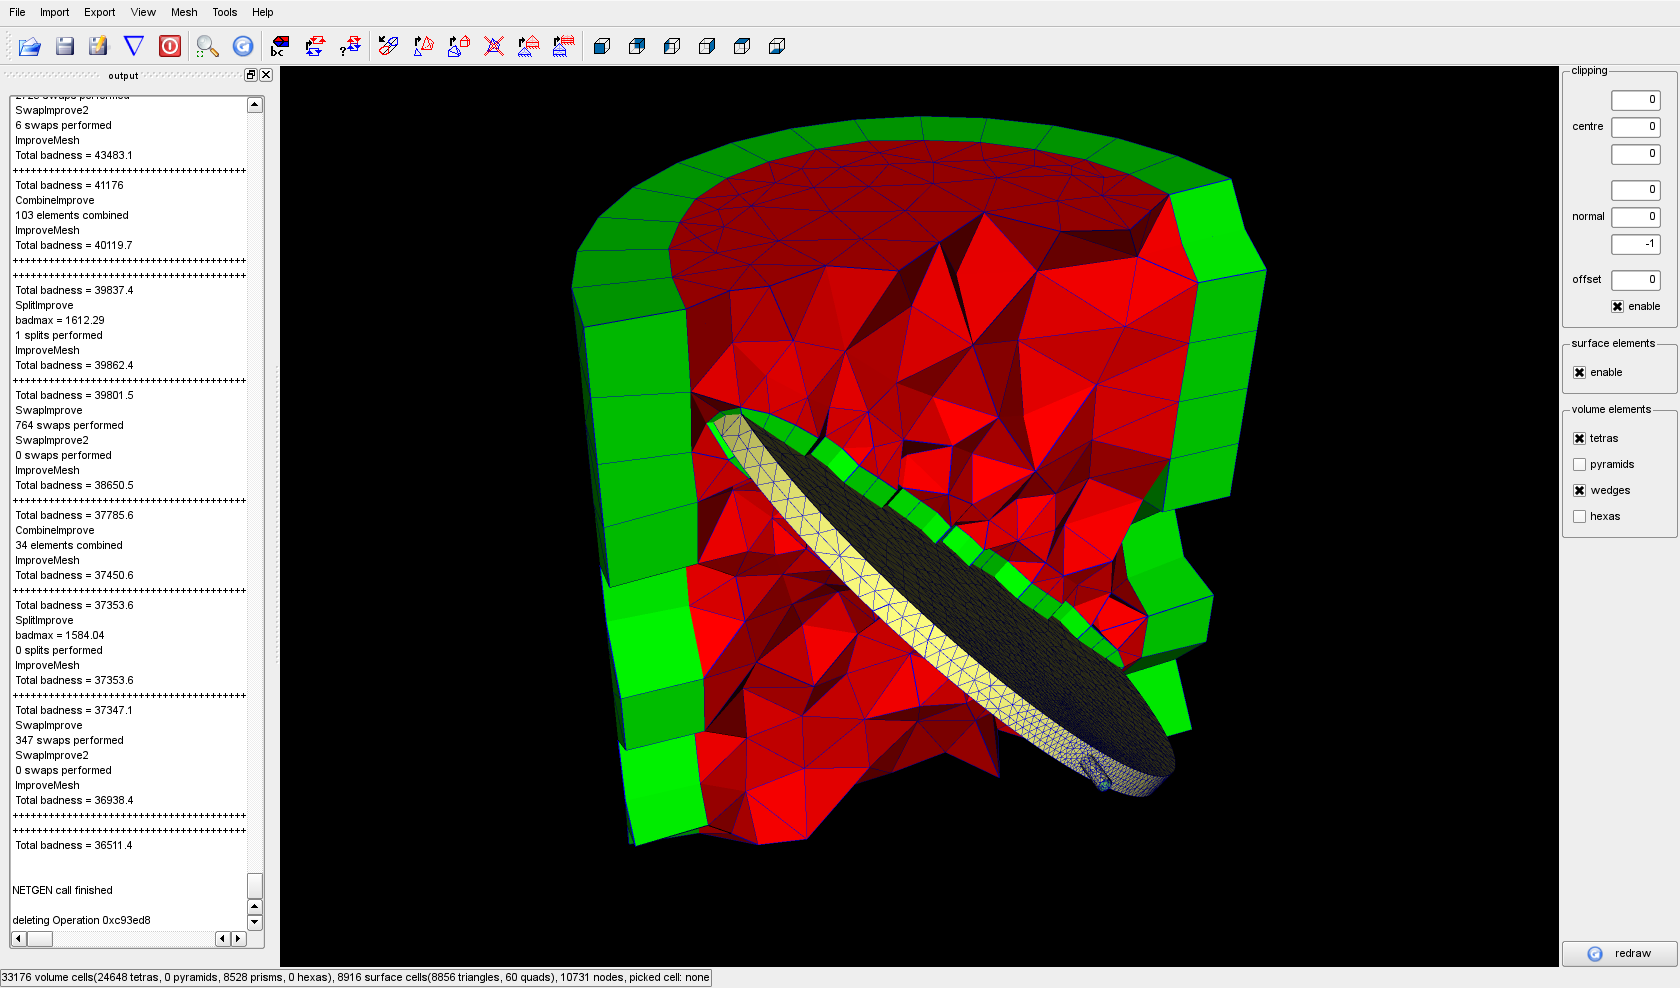
\includegraphics[width=14cm]{figures/tutorials/T1/scr04}
    \par
  \end{centering}
  \caption{First volume grid}
  \label{fig:T1_scr04}
\end{figure}

\clearpage
\subsection{Refining the Boundary-Layer}
At the moment the boundary layer consists of a single layer of prisms. Refining the boundary layer is a straightforward process. 

\important
{
  Save the grid with the refined boundary layer to
  a different file name, or don't save it at all (just export). At the
  moment the refinement cannot be reversed and thus the grid spacing
  cannot be changed. To do this, load the file with the initial one-layer
  boundary layer and refine again.
}

To refine the boundary layer, choose

\menu{Mesh \arr divide prismatic boundary layer}.
\begin{figure}
  \begin{centering}
    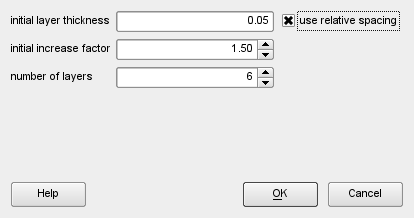
\includegraphics[width=84mm]{figures/tutorials/T1/scr05}
    \par
  \end{centering}
  \caption{Parameters for boundary layer}
  \label{fig:T1_scr05}
\end{figure}

A small pop-up dialogue appears, where you can enter how many layers and how to space them. Relative spacing means, that the initial step size (on the wall) is a fraction of the average local edge length around a node. Absolute spacing uses a fixed distance for all first layer prisms; this will lead to a first layer of prisms which is parallel to the wall. Not all step sizes are possible and \eg will issue a warning if it cannot refine your boundary layer. For this tutorial the settings in figure \ref{fig:T1_scr05} should result in a decent boundary layer mesh.

\clearpage
\subsection{Applying a few Simple Modifications}
\eg offers the possibility to modify the grid by extruding certain boundaries. First we will add a pipe bend by applying a rotational extrusion to the upper boundary (code 3). Afterwards we will add straight sections for the in-flow and out-flow boundaries with the help of a normal extrusion. Please select

\menu{Mesh \arr extrusion}

and enter the parameters exactly as shown in figure \ref{fig:T1_scr06}. After clicking OK you should get a grid like the one shown in figure \ref{fig:T1_scr07}. The extrusion adds a new boundary code (5) which needs to be enabled with

\menu{View \arr boundary codes}

in order to view the newly created geometry. The layer height in figure \ref{fig:T1_scr06} corresponds to an angle in degrees for a rotational extrusion. To extend the pipe at the inlet a normal extrusion with the parameters from figure \ref{fig:T1_scr08} shall be used. If you do the same for boundary code 4 the grid should look like in figure \ref{fig:T1_scr09}. To simplify the later setup of a simulation it is advisable to reset the newly created boundary codes (5,6,8) to the initially set value of 2 for the pipe.

\begin{figure}
  \begin{centering}
    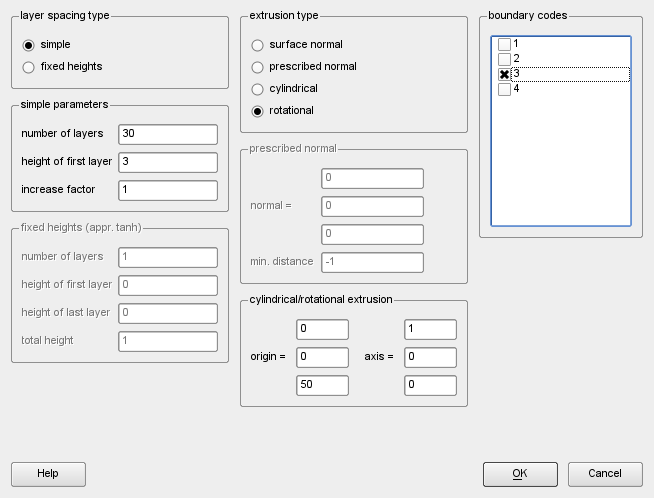
\includegraphics[width=132mm]{figures/tutorials/T1/scr06}
    \par
  \end{centering}
  \caption{Parameters for rotational extrusion}
  \label{fig:T1_scr06}
\end{figure}
\begin{figure}
  \begin{centering}
    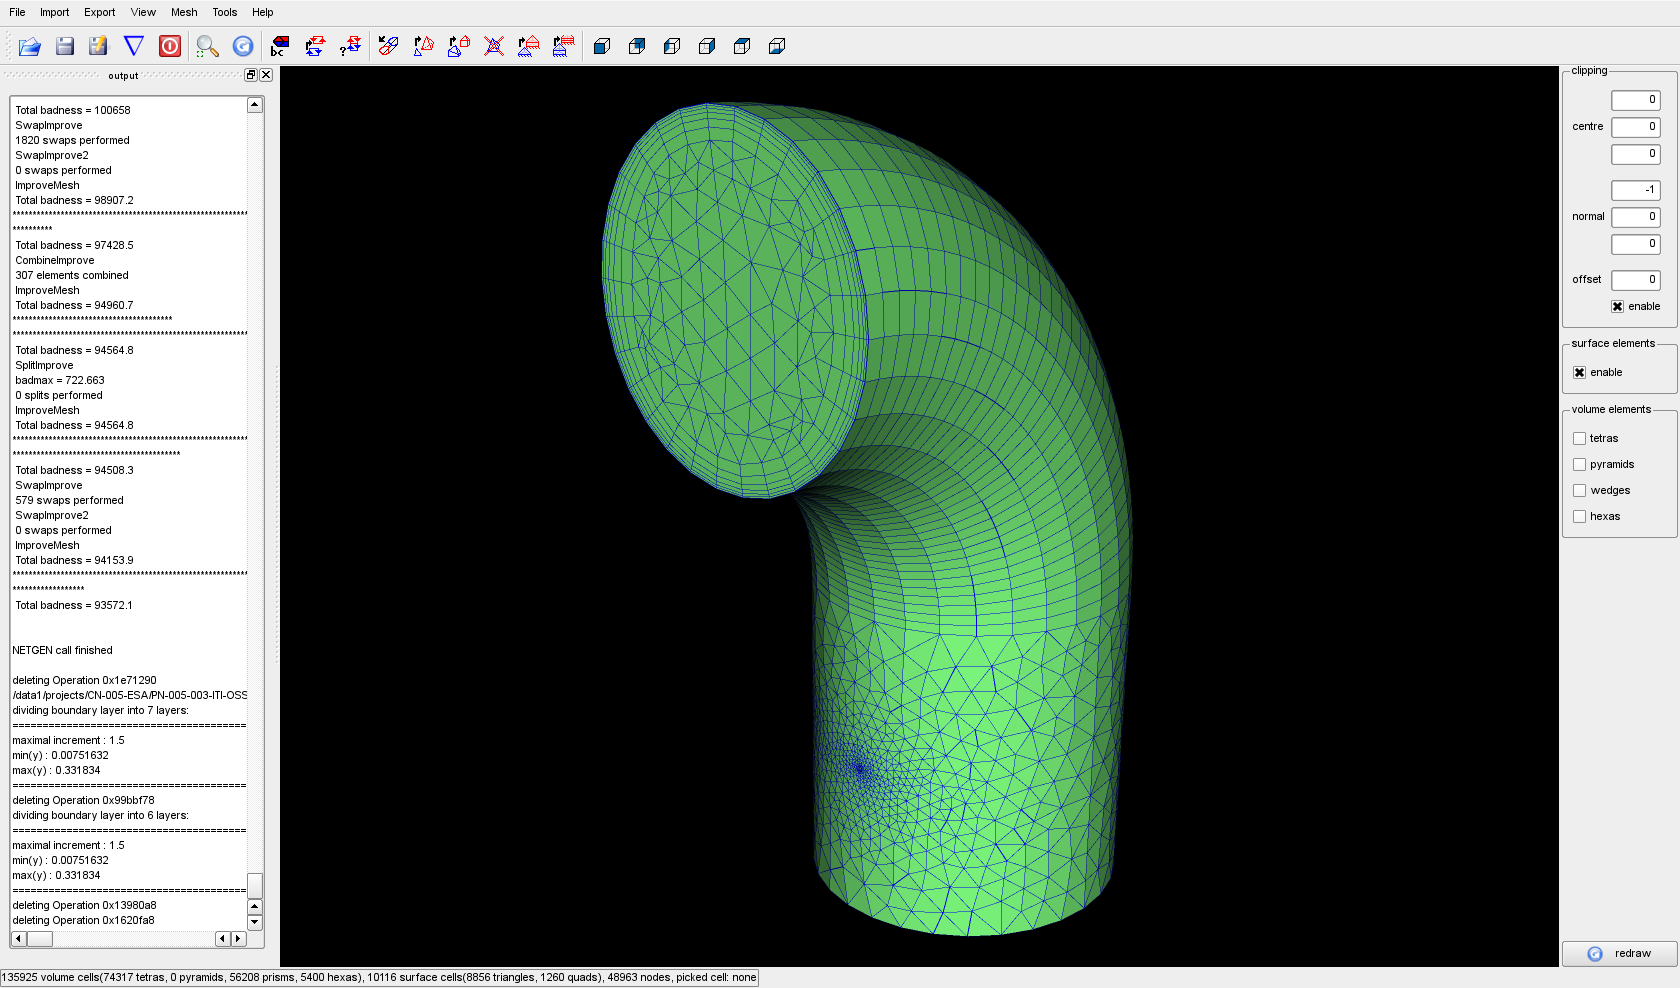
\includegraphics[width=14cm]{figures/tutorials/T1/scr07}
    \par
  \end{centering}
  \caption{Grid after rotational extrusion}
  \label{fig:T1_scr07}
\end{figure}
\begin{figure}
  \begin{centering}
    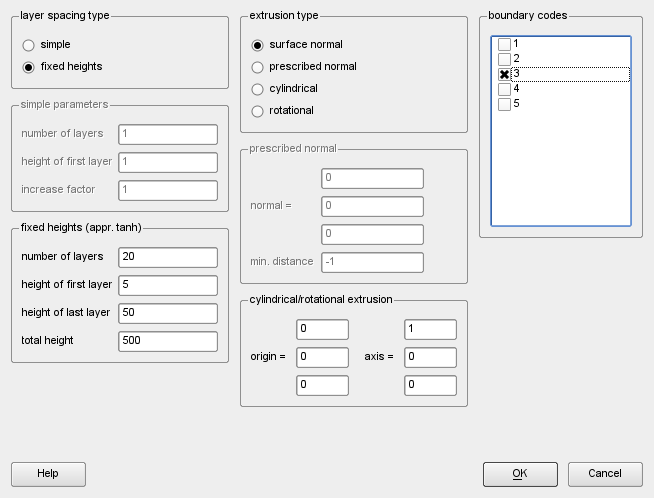
\includegraphics[width=132mm]{figures/tutorials/T1/scr08}
    \par
  \end{centering}
  \caption{Parameters for normal extrusion}
  \label{fig:T1_scr08}
\end{figure}
\begin{figure}
  \begin{centering}
    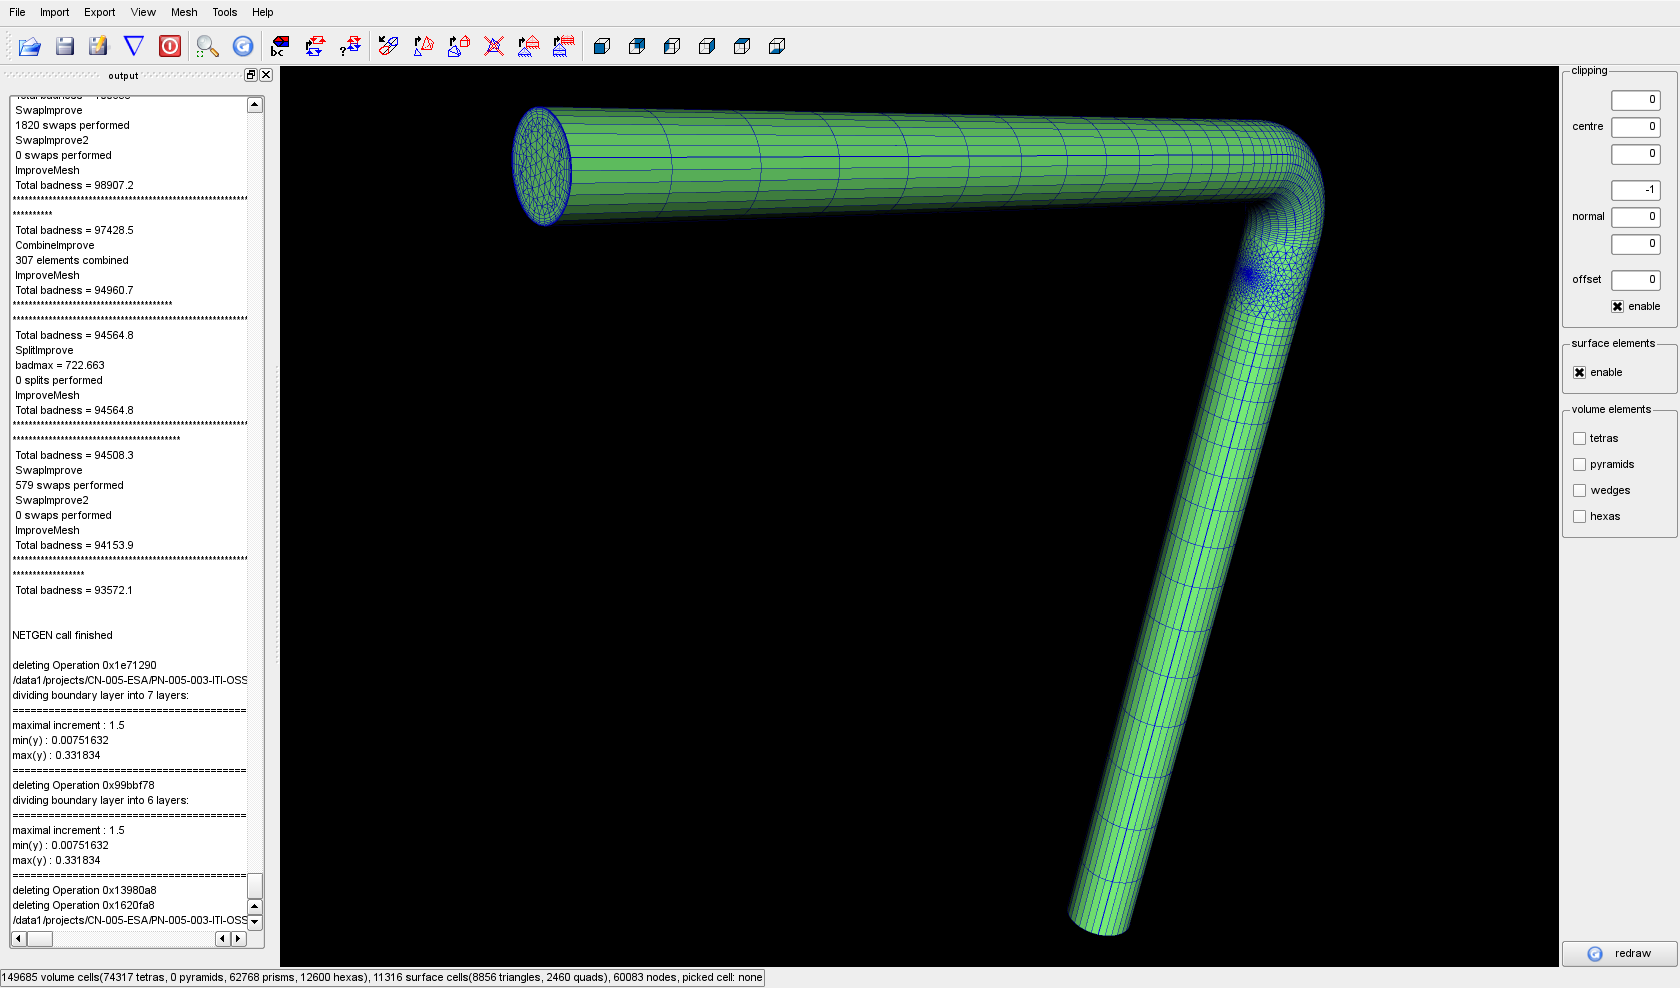
\includegraphics[width=14cm]{figures/tutorials/T1/scr09}
    \par
  \end{centering}
  \caption{Grid after normal extrusion}
  \label{fig:T1_scr09}
\end{figure}
\clearpage

\subsection{Export the Grid to \foam}
Please select

\menu{Tools \arr edit boundary conditions}

and edit the boundary names and types according to figure \ref{fig:T1_scr10}. You can export the mesh using:

\menu{Export \arr OpenFOAM \arr  OpenFOAM}.

This will prompt you for an \foam case directory and the mesh will be directly imported to the \foam format, using the boundary names and types you have defined earlier.

\important
{
  OpenFOAM's checkMesh utility might report a bad mesh
  in case of very thin prisms. A good strategy is to export the mesh
  before the boundary layer is refined, run the checkMesh utility, and
  then - if everything looks alright - refine the boundary layer.
}
\begin{figure}
  \begin{centering}
    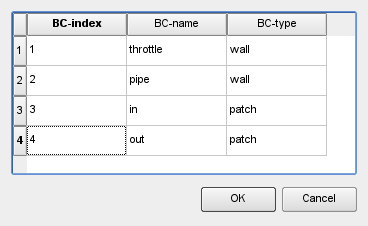
\includegraphics[width=74mm]{figures/tutorials/T1/scr10}
    \par
  \end{centering}
  \caption{Editing the boundary conditions}
  \label{fig:T1_scr10}
\end{figure}

